\section{Synthesis objectives and chosen approach\label{section:inductive-overview}}

This section gives an overview of the synthesis approach. Section~\ref{subsection:inductive-synthesis-statement} states the problem statement in terms of the formal models of Chapter~\ref{chapter:framework}. Section~\ref{subsection:inductive-synthesis-requirements} completes this by stating additional requirements on the synthesis approach. Section~\ref{subsection:inductive-synthesis-approach} presents the grammar induction oriented approach taken in the thesis.

%%%

\subsection{Problem statement\label{subsection:inductive-synthesis-statement}}

In its simplest form, the LTS synthesis problem can be stated as follows:

\begin{quotation}
\noindent \underline{Given}~~a consistent scenario collection showing typical examples and counterexamples of system behaviors

\vspace{-0.7cm}
\begin{align*}
Sc = (S^+,S^-)
\end{align*}

\vspace{-0.2cm}
\noindent \underline{Synthesize}~~the system as a composition of agent LTSs

\vspace{-0.7cm}
\begin{align*}
System = (Ag_1 \parallel \ldots \parallel Ag_n)
\end{align*}

\vspace{-0.2cm}
\noindent \underline{Such that}~~$Sc$ and $System$ are consistent.
\end{quotation}

\noindent For recall, the consistency condition means that (see Section~\ref{subsection:background-scenario-consistency}):

\begin{itemize}
\item \textbf{structural consistency} -- the state machine and scenario views are \emph{structurally} consistent, that is, they agree on the agent decomposition and their respective interface,
\item \textbf{consistent agent views} -- the timelines of any positive scenario $P \in S^+$ specify existing paths in the corresponding agent state machines. The same applies for the precondition of any negative scenario $N \in S^-$.
\item \textbf{consistent system view} -- the system correctly accepts positive scenarios and preconditions of negatives ones. It also correctly rejects negative scenarios. We recall below the precise conditions from Section~\ref{subsection:background-scenario-consistency}:
\begin{align*}
\mathcal{L}(System) &= \mathcal{L}^+(Sc)\\
\mathcal{L}(System) \cap \mathcal{L}^-(Sc) &= \emptyset
\end{align*}

\end{itemize}

%%%

\subsection{Synthesis requirements\label{subsection:inductive-synthesis-requirements}}

The characterization above provides a \emph{minimal requirement} on the synthesis approach. Additional requirements are important to consider as well. Their inclusion depends on assumptions on input scenario models, the presence and/or absence of other models, the availability of an end-user, and so on.

\noindent \textbf{Richness of the scenario language} -- the richness of the input scenario language is an important issue for end-user involvement and usability of a synthesis approach:

\begin{itemize}

\item End-user are most likely to be unable to provide rich scenario descriptions in the early phases of system design. This includes state assertions along scenario episodes or flowcharts on such episodes. The synthesis approach should therefore work when only a few scenarios are available. 

\item Both positive and negative scenarios should be taken into account. Negative scenarios are not uncommon among the examples provided by stakeholders. One reason is that they naturally illustrate violations of safety goals while being easier to specify than the latter.

\item Given the incremental nature of tool-supported system analysis, richer input scenarios are however very likely to be \emph{eventually} available. Higher-level scenario models should therefore be supported as input of the synthesis technique for advanced analysis phases.

\end{itemize}

\noindent \textbf{Behavior generalization} -- the synthesis approach must at least cover the behaviors described in the positive scenarios. In most cases, scenarios provide \emph{examples} of system behaviors and are inherently incomplete. Synthesized state machines should therefore cover more behaviors than those already described. 

An upper bound on behavior generalization is entailed by the consistency condition, that requires negative scenarios to be correctly rejected. This upper bound has to be refined when other models are available (see below).

\noindent \textbf{Multi-model consistency} -- A argument similar to the one for high-level scenario models applies for other models. Fluents, goals and domain properties, etc. should not be \emph{required} as input, but are better \emph{supported} when available. 

In presence of multiple models, strengthening the characterization above is required. All available models shall be required to be consistent in input. In that case, the synthesis technique shall be such that synthesized LTSs are consistent with all input models. Notably, the synthesized system should not violate known safety goals.

%%%

\subsection{A grammar induction approach\label{subsection:inductive-synthesis-approach}}

Figure~\ref{image:inductive-synthesis-overview} shows the three main steps of our synthesis approach. We will assume here that a scenario collection $Sc = (S^+, S^-)$ is taken as input of the synthesis process. Adaptations of the first two steps below are required to take high-level MSCs as input; they will be covered in Section~\ref{section:inductive-from-hMSC}.

\begin{figure}\centering
  \scalebox{0.60}{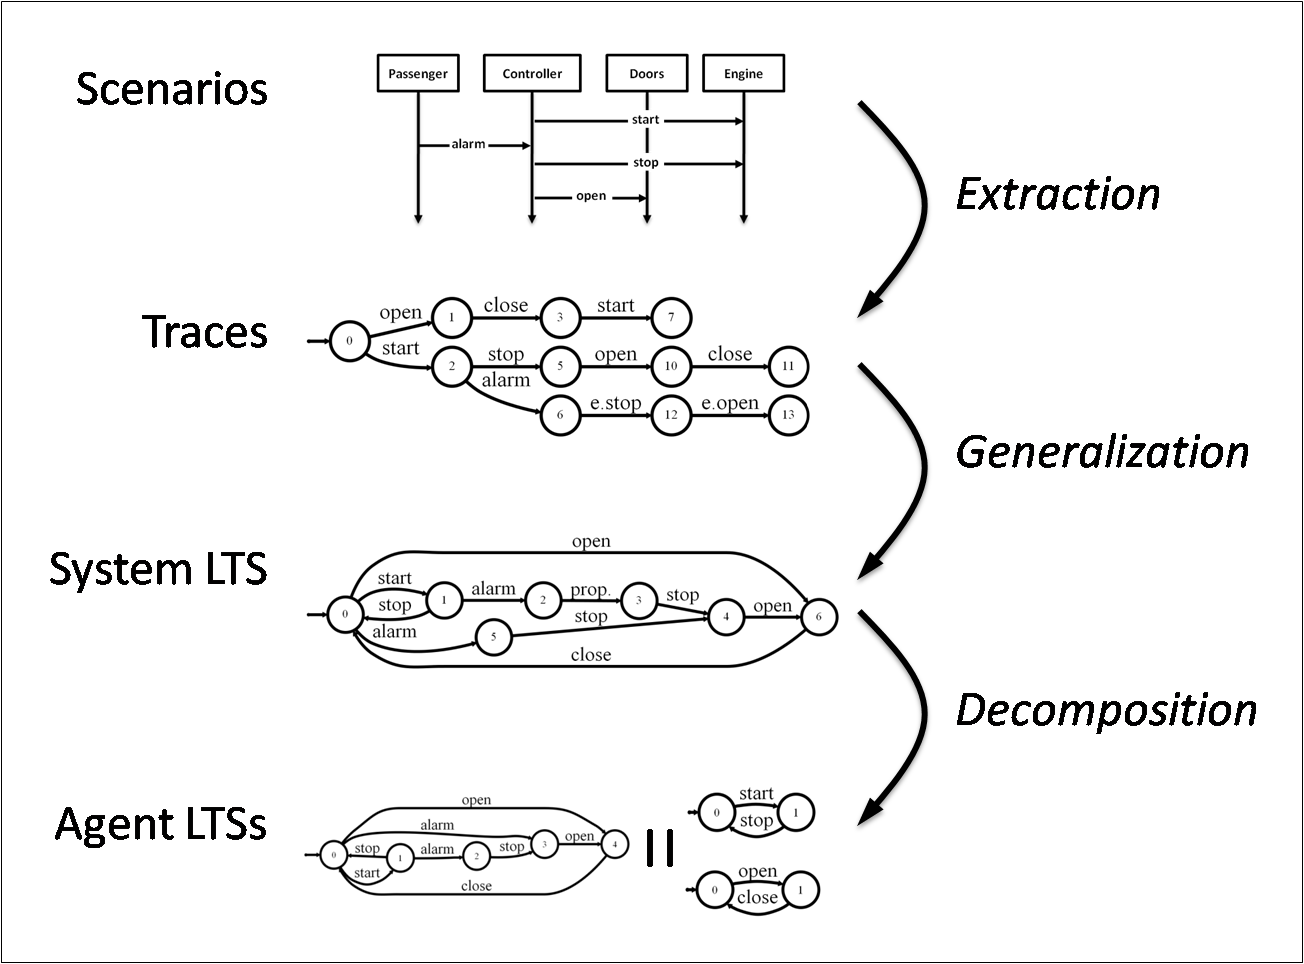
\includegraphics[trim=2mm 2mm 3mm 2mm, clip]{src/4-inductive/images/overview}}
  \caption{Overview of inductive LTS synthesis from MSCs.\label{image:inductive-synthesis-overview}}
\end{figure}

\noindent \textbf{Extraction} -- this step consists in extracting scenarios traces as a first automaton. The extraction relies on the trace semantics of scenarios given in Chapter~\ref{chapter:framework}. 

Traces are captured by a \emph{prefix tree acceptor} (PTA), the largest deterministic automaton that exactly accepts the positive behaviors. At this step, the \artifact{consistent system view} condition already holds, but no generalization occurs yet:
\begin{align*}
\mathcal{L}(PTA) &= \mathcal{L}^+(Sc)\\
\mathcal{L}(PTA) \cap \mathcal{L}^-(Sc) &= \emptyset
\end{align*}

\noindent \textbf{Generalization} -- grammar induction is used at this step so as to fullfil the behavior generalization requirement. The Regular Positive and Negative Inference (RPNI) algorithm is used as a building block \cite{Oncina:1992} for synthesizing a system LTS from the PTA.

Roughly, this algorithm incrementally refines a current automaton solution by merging well selected state pairs; the generalization is performed under the control of negative scenarios. The \artifact{consistent system view} remains an invariant for any current solution $A$:
\begin{align*}
\mathcal{L}(A) &\subseteq \mathcal{L}^+(Sc)\\
\mathcal{L}(A) \cap \mathcal{L}^-(Sc) &= \emptyset
\end{align*}

This inductive approach is enhanced in two ways so as to fulfill additional requirements:

\begin{itemize}

\item An interactive feature supports the elicitation of additional, ``interesting'' scenarios that are not originally provided by the end-user. The latter is expected to classify generated scenarios as positive or negative system behaviors. This feature helps iteratively enriching the available scenario models.

\item Fluents, legacy components and goals can be injected in the generalization process when available. In addition to guaranteeing multi-model consistency, taking such models into account helps pruning the induction search space.

\end{itemize}

\noindent \textbf{Decomposition} -- the decomposition step computes an LTS for each agent by projecting the system LTS on their respective alphabet. For an agent $Ag$ the projection of the system LTS $S$ is given by:
\begin{align}
(S \setminus \Sigma_{Ag}^c)^\Delta
\end{align}
\noindent where $\Sigma_{Ag}^c$ denotes the set of all system events but those of $Ag$'s interface.

This step guarantees that the \emph{structural consistency} and \emph{consistent agent view} conditions hold.

The extraction and decomposition steps are straightforward applications of the material given in Chapter~\ref{chapter:framework}. The rest of this chapter therefore focusses on the generalization step achieved through grammar induction. The next section provides background on grammar induction and the RPNI algorithm.
